\documentclass[11pt, letterpaper]{article}
\usepackage[utf8]{inputenc}
\usepackage[letterpaper, margin=1in]{geometry}
\usepackage{amsmath}
\usepackage{amssymb}
\usepackage{amsthm}
\usepackage{graphicx}
\usepackage[font=scriptsize]{caption}
\usepackage{subcaption}
\graphicspath{ {.} }
\captionsetup{justification=raggedright, singlelinecheck=false}


\title{Homework 2}
\author{Ryan Tang}
\date{September 29th 2022}

\begin{document}
\maketitle

\section{Exercise 10.1}
Since $G$ is the minimal I-map for $p(A, B, C, D, E, F, X)$, no other subgraph $G^{\prime}$ should contain any additional conditional-independence (CI) statements. Here, given the graph $G$, both $E$ and $F$ are independent of $A$ and $B$ given $X$. After marginalize out $X$, we need to add edges for $A \rightarrow E$, $B \rightarrow E$, $A \rightarrow F$, and $B \rightarrow F$. Otherwise, we will create an independence statement like $A \perp E$, which was not a part of the minimal I-map $G$.

\begin{figure*}[!h]
  \centering
  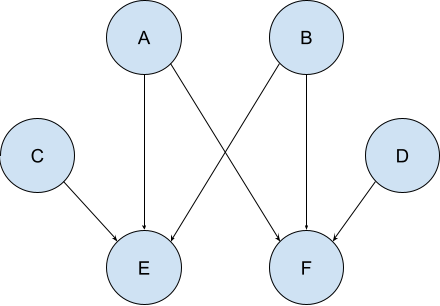
\includegraphics[width=0.4\textwidth]{hw2/10.1.png}
  \captionsetup{justification=centering}
  \caption{The new graph}
\end{figure*}

\section{Exercise 10.2}
\paragraph{(a)} Only $D$ is conditionally independent of $A$ given $B$; other nodes are not completely d-separated by B.
\paragraph{(b)} $\{C, E, F, H, I\}$ are conditionally independent of $A$ given $J$. Knowing $J$ opened the path between $A$ and $\{D, B\}$ instead.

\section{Exercise 10.3}
Given a graph $G$ with $V$ nodes, $t \in V$, $x_t$ is one of the node. And say $X_{-t}$ contains the set of nodes that consists of the Markov Blanket, $mb(x_t)$ of nodes $x_t$. Here we proof the full conditional of the Markov Blanket of node $x_t$ is given the following. Note, here we are only assuming the first-order Markov property within a DAG context.
\begin{proof}
\begin{align*}
    p(x_t|X_{-t}) &= \frac{p(x_t, X_{-t})}{p(X_{-t})} \\
        &\propto p(x_t, X_{ch(t)}, X_{pa(t)}, X_{copa(t)}) \\
        &= (\prod_{i \in pa(t)} p(x_i)) \cdot p(x_t|X_{pa(t)}) \cdot \prod_{j \in ch(t)} p(x_j|X_{pa(j)}) \\
        &\propto p(x_t|X_{pa(t)}) \cdot \prod_{j \in ch(t)} p(x_j|X_{pa(j)})
\end{align*}
\end{proof}

\section{Exercise 10.4}
\paragraph{(a)}
For nodes $X_{1:3}$, we only need one parameter for each to encode the binary outcome, 3 here. The hidden node needs one parameter per any possible combination of outcomes from $X_{1:3}$, $2^3=8$. For nodes, $X_{4:6}$, each of them needs one parameter for each possible outcome from the hidden node, $3*2=6$. Hence, we have $17$ parameters in the latent variable model.

\paragraph{(b)}
In contrast, the fully observed model with latent variable requires $59$ parameters because of the following: 1 parameter for each node in $X_{1:3}$. Node $X_4$ has 3 parents; thus, a table of $2^3=8$ parameters. Node $X_5$ has 4 parents, which requires a table of $2^4=16$ parameters. Lastly, node $X_6$ has 5 parents, which requires a table of $2^5=32$ parameters.

\paragraph{(c)}
The latent variable model is usually preferred because it has less number of parameters to estimate and can be estimated using the EM algorithm and MLE through MLE. It becomes more true when $n$ is small. However, it is all assumed that the latent variable model is a good representation of the underlying process.


\section{Exercise 10.5}
\paragraph{(a)}
\begin{align*}
    p(S=1|V=1) &= \frac{p(S=1, V=1)}{p(V=1)} \\
        &= \frac{p(V=1) \sum_i p(S=1|G=g_i)p(G=g_i)}{p(V=1)} \\
        &= \sum_i p(S=1|G=g_i)p(G=g_i) \\
        &= (1-\gamma)\alpha + (1-\beta)(1-\alpha)
\end{align*}

\paragraph{(b)}
$p(S=1|V=0)$ is equal to $p(S=1|V=1)$ because $V$ and $S$ are conditionally independent with each other as long as $R$ is not observed.

\paragraph{(c)}
The MLE result is $\delta=0, \alpha=\frac{1}{3}, \beta=0, \gamma=1$


\end{document}